% 
% Annual Cognitive Science Conference
% Sample LaTeX Paper -- Proceedings Format
% 

% Original : Ashwin Ram (ashwin@cc.gatech.edu)       04/01/1994
% Modified : Johanna Moore (jmoore@cs.pitt.edu)      03/17/1995
% Modified : David Noelle (noelle@ucsd.edu)          03/15/1996
% Modified : Pat Langley (langley@cs.stanford.edu)   01/26/1997
% Latex2e corrections by Ramin Charles Nakisa        01/28/1997 
% Modified : Tina Eliassi-Rad (eliassi@cs.wisc.edu)  01/31/1998
% Modified : Trisha Yannuzzi (trisha@ircs.upenn.edu) 12/28/1999 (in process)
% Modified : Mary Ellen Foster (M.E.Foster@ed.ac.uk) 12/11/2000
% Modified : Ken Forbus                              01/23/2004
% Modified : Eli M. Silk (esilk@pitt.edu)            05/24/2005
% Modified : Niels Taatgen (taatgen@cmu.edu)         10/24/2006
% Modified : David Noelle (dnoelle@ucmerced.edu)     11/19/2014

%% Change "letterpaper" in the following line to "a4paper" if you must.

\documentclass[10pt,letterpaper]{article}

\usepackage{cogsci}
\usepackage{pslatex}
\usepackage{apacite}
\usepackage{url}
\usepackage{graphicx}
\usepackage{caption}
\usepackage{listings}
\usepackage{color}
\usepackage{textcomp}

\graphicspath{{figures/}}

\def\signed #1{{\leavevmode\unskip\nobreak\hfil\penalty50\hskip2em
  \hbox{}\nobreak\hfil(#1)%
  \parfillskip=0pt \finalhyphendemerits=0 \endgraf}}

\newsavebox\mybox
\newenvironment{aquote}[1]
  {\savebox\mybox{#1}\begin{quote}}
  {\signed{\usebox\mybox}\end{quote}}


\lstset{
  language=Scheme, % Andreas Stuhlmuller. Scheme listings. https://github.com/stuhlmueller/scheme-listings.git
  columns=fixed,
  tabsize=2,
  extendedchars=true,
  breaklines=true,
  frame=single,
%  numbers=left,
  numbersep=5pt,
   basicstyle=\scriptsize\ttfamily
%  rulesepcolor=\color{solarized@base03},
%  numberstyle=\tiny\color{solarized@base01},
%  keywordstyle=\color{solarized@green},
%  stringstyle=\color{solarized@cyan}\ttfamily,
%  identifierstyle=\color{blue},
%  commentstyle=\color{solarized@base01},
%  emphstyle=\color{solarized@red}
}

\definecolor{Red}{RGB}{255,0,0}
\newcommand{\red}[1]{\textcolor{Red}{#1}}  


\title{Generic meanings are vague but rationally inferred from context}
 
 \author{{\large \bf Michael Henry Tessler, Noah D. Goodman } \\
	\{mhtessler, ngoodman\}@stanford.edu \\
  Department of Psychology, Stanford University}
 
\begin{document}

\maketitle


\begin{abstract}
Insert abstract here.

\textbf{Keywords:} 
generics; pragmatics; bayesian cognition; bayesian data analysis
\end{abstract}

\begin{aquote}{Barack Obama, \emph{2015 State of the Union Address}}
New sanctions passed by this Congress, at this moment in time, will all but guarantee that diplomacy fails -- alienating America from its allies; making it harder to maintain sanctions; and ensuring that Iran starts up its nuclear program again.
\end{aquote}


Generic meanings are hard to pin down.  Consider President Obama's remark during the State of the Union Address. The sentence is a generic statement about \emph{new sanctions} in that it conveys a generalization about the members of a kind \cite{Carlson1977, Leslie2008}. It invites the question: ``Exactly how many of these new sanctions will guarantee diplomacy fails?'' President Obama's statement is conceivably true for a range of possible values. At the same time, he is not a man to waste words, and so why does he go through the trouble of saying such a statement? In this paper, we will see that both the context in which his words are uttered and his effort in producing this statement contribute to the meaning we derive. % 

Generic statements are puzzling because they accommodate a range of quantification. On one hand, generics would seem to suggest an almost universal quantification, as in ``Dogs bark''. Others, like ``Mosquitos carry West Nile virus'', express a relation that applies only to a small subset of the kind. It is perhaps this inherent uncertainty that leads generics to be so widespread in natural language. 

\citeA{Cimpian2010} (henceforth, CBG) carried out a series of controlled studies designed to examine the truth conditions and implications of generic statements. They found consistent evidence that the generic is interpreted more strongly than one would expect based on its truth conditions. The authors also found evidence for the influence of context on participants' willingness to accept the relevant generics (i.e. context modified the truth conditions). 

In their \emph{truth conditions} task, participants were given an evidence statement in terms of the percentage of a category that had a property (e.g. ``30\% of lorches have purple feathers.''). Participants were asked whether the associated generic statement (i.e. ``Lorches have purple feathers'') was true or false. The authors manipulated context within-subjects by adding additional statements about the property. Three contexts will focus on in this paper are \emph{dangerous and distinct} (DD), \emph{not distinct and irrelevant} (NI), and \emph{plain} (P). The authors found that DD increased the overall proportion of ``true'' responses of the generic propositions. That is, when the property in question was dangerous and distinct, participants required a lower overall prevalence (e.g. when 10\% or 30\% of lorches had purple feathers) to assert that the generic statement was true.

In their \emph{implied prevalence} task, participants were supplied with the generic (still, with context as a within-subjects variable) and asked ``What percentage of lorches do you think have purple feathers?''. The authors consistently found that the generic was interpreted as referring to nearly all lorches. 

This contextual effects on truth conditions and the asymmetry between verification and interpretation pose a puzzle for formal semantics. In this paper, we seek to explain both of these phenomena in terms of pragmatic inference arising from a vague statement. We draw on new advances in probabilistic pragmatics to formalize two possible theories of the generic. Further, we harness the power of Bayesian data analysis to mediate between these formal theories and draw inferences about cognitively interesting model parameters. 


%(e.g. ``These feathers are as sharp as needles and can easily get lodged in you, causing massive bleeding. No other animals have these kinds of feathers'')
% (e.g.  ``These feathers are wide and very smooth to the touch. Other animals have these kinds of feathers.'')

%How are we to understand these data? One interpretation is that context changes the truth-conditions for a generic statement, but that within a context, the truth-conditions are stable. A different sort of explanation is that context changes the nature of world somehow, and that generic meanings are inferred rationally from context. We draw on recent advances in probabilistic pragmatics and Bayesian data analysis to mediate between these two alternatives.


\section{Experiment 1: CBG (Exp. 1) replication}

Experiment 1 attempted to replicate the finding of CBG Exp. 1 that context affects the proportion of ``true'' responses to a generic statement. 

\subsection{Method}

\subsubsection{Participants}

We recruited 40 participants over Amazon's crowd-sourcing platform Mechanical Turk. 

\subsubsection{Procedure and materials}

Our procedure was very similar to CBG \emph{truth conditions} task. Our instructions were elaborated to improve interest and motivation\footnote{The experiment in full can be viewed at \url{http://stanford.edu/~mtessler/experiments/generics/cbg2010-replication/experiment/experiment-9.html}}. 

We used the same materials as CBG (available in their Appendix). The materials used were 30 novel animals (e.g. lorches, morseths, blins) each paired with a unique property. Properties were pairs of colors and body-parts (e.g. purple feathers, orange tails). Each participant saw unique 10 animal-property pairs in each of 3 contexts \{\emph{plain}, \emph{DD}, \emph{NI}\}. Those 10 items were randomly paired with 1 of 5 ``prevalence levels'': \{10, 30, 50, 70, 90\}\%; each prevalence level appeared 2 times per context. 

Participants saw a prevalence statement and a context. A context here was either (1) dangerous \& distinct statements (e.g. ``These feathers are as sharp as needles and can easily get lodged in you, causing massive bleeding. No other animals have these kinds of feathers.''), (2) not distinct \& irrelevant statements (e.g. ``These feathers are wide and very smooth to the touch. Other animals have these kinds of feathers.'', or (3) nothing else. Participants were then asked ``Is the following sentence true or false?'', below which was presented the associated generic (e.g. ``Lorches have purple feathers'') and 2 radio buttons. 

\subsubsection{Results}

\begin{figure}
\centering
    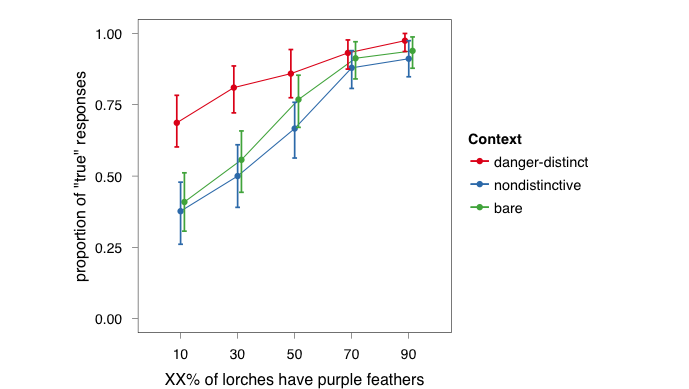
\includegraphics[width=\columnwidth]{fig1_replication}
    \caption{Replication of CBG Exp. 1, generics condition}
  \label{fig:replication}
\end{figure}


Our results replicated the finding of CBG that the generic statement was endorsed more in the dangerous and distinctive context than in the other two contexts (Figure \ref{fig:replication})\red{[insert stats here]}. There was also an interaction between prevalence level and context such that the DD context was endorsed more particularly at lower prevalence levels. \red{[insert stats here]}. 

\section{Bayesian analysis of fixed-threshold semantics}

These statistics tell us that there were significantly more ``true'' responses in one context vs. another, and that these relative proportions of ``true'' responses were most different at the lower prevalence levels (via the interaction term of the regression). What we'd really like to know, however, is how the truth-functional threshold of the generic behaves across these three contexts. To do this, we have to move beyond Null Hypothesis Significance Teseting to do Bayesian inference over the unknown threshold of generic. The data analysis model can be written very simply in Church \cite{probmods}.

\begin{lstlisting}
(define bayesian-data-analysis 
	(query
		; we don't know the generic threshold but we feel it might be a function of context
		(define generic-threshold 
			(lambda (context) (uniform 0 1)))
		; a generic statement is true if the prevalence of the property is greater than threshold
		(define generic 
			(lambda (prevalence context) 
				(> prevalence (generic-threshold context))))
		
		(define phi (uniform 0 1)); guessing parameter
				
		generic-threshold ; return generic-threshold	
		
		(= experiment1-data 	; condition on exp.1 data 
			(if (flip phi) ; IF participant is guessing
				   (flip 0.5) ; then they guess
				   (generic prevalence context))))) ;otherwise, they evaluate the generic
\end{lstlisting}

The model above is a data analysis model to try to infer the threshold of the generic, with the built-in flexibility that it might vary by context. There is an implicit cognitive model here (hidden in \lstinline{generic} function). It says the generic is like an alien quantifier. This quantifier behaves like other quantifiers in that it has a fixed-threshold semantics. The only thing special about the generic is that the threshold might be different for different contexts. 

We don't know what the generic might mean \emph{a priori}. Thus, the generic-threshold\footnote{If the generic threshold turns out to be 0, the generic ``Lorches have purple feathers'' would mean essentially, ``Some lorches have purple feathers''. If the threshold turned out to be very close to 1, the generic would mean essentially: ``All lorches have purple feathers''.} follows a uniform prior distribution between 0 and 1. The generic, here, is assumed to have a truth-functional meaning such that it is \lstinline{true} when the prevalence is over \lstinline{generic-threshold}, and false when it is not. We include the data-analytic parameter \lstinline{phi} to account for data points that deviate strongly from our theory; it is a guessing parameter. We assume there is some proportion of responses\footnote{Ideally, we would have \lstinline{phi} be a function of participant (some participants guess more than others) and experimental condition (some conditions are more difficult or less constrained and invite more guessing). As a first pass, we assume there is some global quantity of guessing.} where the participant is responding randomly, and we estimate this quantity by way of \lstinline{phi}.

The \lstinline{query} function is written to return \lstinline{generic-threshold}, which is the parameter we are interested in inferring. Finally, the last line is our condition statement: we condition on the data we collected in Experiment 1, which could either be generated from our theory (that \lstinline{prevalence} is greater than \lstinline{generic-threshold}) or by guessing (via \lstinline{phi}). 

\subsection{Results}
\begin{figure}
\centering
    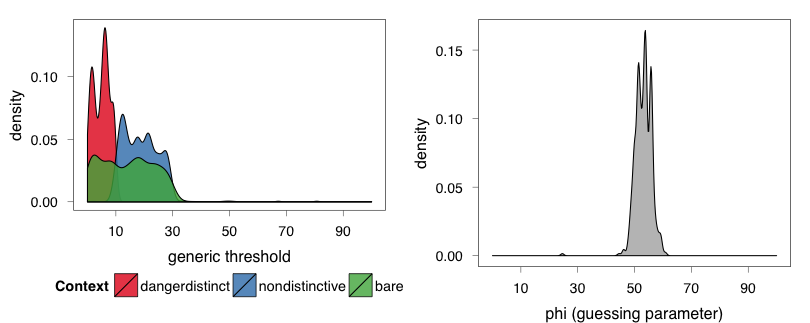
\includegraphics[width=\columnwidth]{fig2_bda1_combined}
    \caption{Inferred threshold for the generic across contexts}
  \label{fig:bda1a}
\end{figure}

The results can be seen in Figure \ref{fig:bda1a}. In the \emph{plain} condition, the analysis suggests the threshold is somewhere between 0\% and 30\%, but it's unclear where exactly in that range the threshold should be\footnote{This uncertainty results from the sparseness of our sampling (see Procedures and Materials). Participants were queried only at prevalence levels 10, 30, 50, 70, and 90}. Critically, in the \emph{dangerous and distinctive} context, the analysis infers a lower threshold, less than 10\%. This matches with intuition and the empirical results, that a dangerous and distinctive context allows for the generic to be more permissive (e.g. ``Mosquitos carry West Nile Virus'' is true, even though very few mosquitoes actually do). Finally, and most intriguingly, the analysis infers a third distinct threshold profile for the \emph{nondistinct and irrelevant} context.  For this, it says that threshold is greater than 10\%, but could be as high as 50\%. This is an overall higher inferred threshold for the nondistinctive category and an aspect of analysis totally obscured by standard frequentist estimation. 

This model is too a simple model, however. We see this in part by the posterior distribution of the data analysis parameter \lstinline{phi}. This parameter is one measure of fit because it represents the percentage of responses that the data analysis model wants to attribute to guessing. With this cognitive model, the percentage of guesses is somewhere between 40\% and 50\%. The amount of guessing is so high because our computational model is inflexible.

This can also be seen in the posterior predictive distribution of responses (Figure \ref{fig:bda1posteriorpred}, left). The model matches the ordering of the truth-conditions by context reasonably well, but is too dichotomous in its predictions. The correlation between the posterior predictive and the data is $r = 0.81$. 

\begin{figure}
\centering
    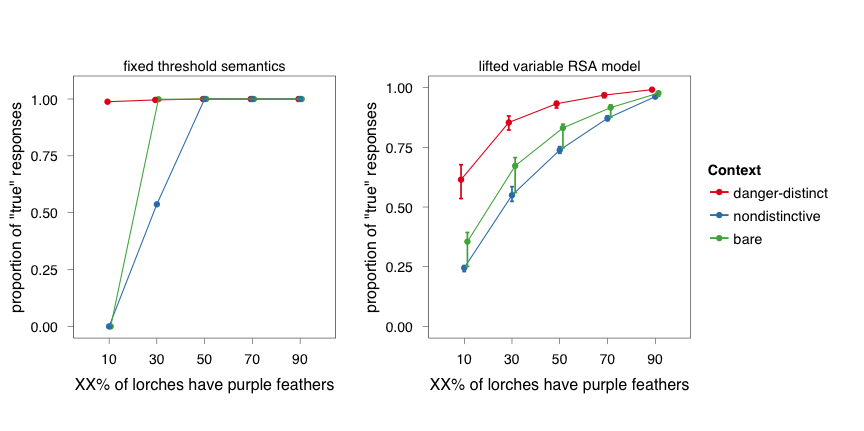
\includegraphics[width=\columnwidth]{fig3_2pps}
    \caption{Posterior predictive using fixed-threshold semantics (left) and lifted-variable (RSA) right.}
  \label{fig:bda1posteriorpred}
\end{figure}

%\begin{itemize}
%\item Inferred value of theta across contexts. 
%\item $\phi$ parameter. 
%\item Posterior predictive of fixed threshold model?
The problem with this approach is that we are assuming there is some threshold for the generic, out there in the world, and that all there is to do is go out and measure it. An alternative is to consider that there is indefeasible uncertainty about the threshold, but that listeners try their best and actively infer, from context, probable values of the threshold. To express this type of model, we must consider the pragmatics of language understanding. 

%\end{itemize}

\section{Lifted-variable RSA}

The bayesian data analysis above provides evidence that context influences the truth-conditions of a generic statement. The poor qualitative fit as well as the inferred value of the guessing parameter \lstinline{phi} suggest, however, that our model of cognition is incomplete. Rather than propose that the meaning of a generic is simply a one-to-one mapping between context and threshold, we propose people have uncertainty about the true threshold and actively reason about this meaning from interaction and context. 

To formalize this, we draw on work from the Rational Speech-Act (RSA) theory of language understanding \cite{Frank2012}. In this framework, a listener infers the meaning of an utterance by a recursive reasoning process, wherein she considers the thought-processes of a speaker whose goal is to be informative. This theory has gained tremendous support for providing computational explanations for a number of linguistic phenomena including scalar implicature, hyperbole, and multiple classes of reasoning paradigms \cite{Goodman2013, Kao2014, Tessler2014, Lassiter2014}. 

RSA has recently been extended to accommodate words that don't have fixed semantics. \citeA{Lassiter2015} proposed an elaboration of the theory to account for interpreting vague, gradable adjectives like \emph{tall}. They propose the meaning of an adjective like \emph{tall} is a standard truth-functional meaning such that the adjective is true if the object in question has a height greater than the threshold $\theta_{tall}$. The suggestion, though, is that the listener has uncertainty about what $\theta_{tall}$ actually is, and infers that value of $\theta_{tall}$ via the same recursive reasoning process. Here, we borrow the same formalism to try account for the uncertainty in generic meaning.

In Church, the model looks like:

\begin{lstlisting}
(define pragmatic-listener (lambda (utterance)
	(query
		(define state (state-prior))
		(define theta (theta-prior))
			
		state
			
		(equal? utterance (speaker state theta)))))
			
(define speaker (lambda (state theta)
	(query
		(define utterance (utterance-prior))
			
		utterance
			
		(equal? state (literal-listener utterance theta)))))
			
(define literal-listener (lambda (utterance theta)
	(query
		(define state (state-prior))
			
		state
			
		(utterance state theta))))
\end{lstlisting}

This is a model of a listener who has been told a generic statement. The listener is pragmatic, insofar as she doesn't know what the world is like, or even what the generic means in the sense of its semantic content. She assumes, however, that the speaker was trying to be informative and that his goal was to communicate the true state of the world. From this, the listener jointly infers both the \lstinline{state} and the threshold \lstinline{theta}. We call this type of model a ``lifted variable'' model because \lstinline{theta}, traditionally thought to be part of the semantic content of the utterance and thus perfectly transparent to all in the conversation, has been ``lifted'' to the pragmatic level and must be inferred like \lstinline{state}.

The CBG truth conditions task is not a task for a listener, however, but for a speaker \footnote{See \citeA{Degen2014} for an exposition on how dependent measures map onto different roles in communication.}. Thus, we must say that the there is a speaker, who reasons about the pragmatic-listener, who is trying to infer the state and theta and so on. Our final piece to the cognitive model looks like:

\begin{lstlisting}
(define rational-speech-act

	(define lifted-speaker (lambda (state)
		(query
			(define utterance (utterance-prior))
			
			utterance
			
			(equal? state (pragmatic-listener state)))))	
			
	(define pragmatic-listener (lambda (utterance)
		...)))
\end{lstlisting}

The speaker here, doesn't even consider what the threshold might be, but knows that the pragmatic listener is thinking about it, and so will tailor his utterance appropriate.

\subsection{Inferring a threshold}

How is a listener supposed to reason about the threshold? In the case of adjectives, reasonable thresholds are determined the prior in question. If we say ``John is tall'' and the ``Empire State Building is tall'', then the inferred cut-off for these two statements will be informed by the prior distribution of heights for people and buildings, respectively. 

We propose that in this paradigm, the threshold is influenced via the contextual information given. In CBG, this contextual information amounts to the 3 experimental conditions: \emph{dangerous and distinct}, \emph{nondistinct}, and \emph{bare}. In this simple model, the contextual information could provide different \lstinline{state-prior} distributions. \lstinline{state-prior} represents the  prior probability that some percentage of the kind has the property. Naively, this would be \lstinline{(uniform 0 1)}, or equivalently \lstinline{(beta 1 1)}. However, we propose that the participant has different prior distribution in mind, depending on relevance of the properties under discussion (given, again, but the experimental conditions).

\subsection{Inferring a prior}
We, as scientists, don't know what these prior distributions look like (although we might have some intuitions). Thus, we put uncertainty over the parameters of this beta distribution, \lstinline{(beta gamma delta)}\footnote{For ease of interpretation, we are parametrizing the \lstinline{beta} distribution by its mean and some measure of its variability ... \lstinline{(beta (* gamma delta) (* (- 1 gamma) delta))}}, outside of the RSA model but inside of the data analysis model. 

Thus, we put a bayesian data analysis model on top of a Rational Speech-Act model of language understanding, to see how context might influence the prior distribution given the data we've observed. We keep the data-analytic guessing parameter \lstinline{phi} as a gross estimate of the proportion of responses our model of cognition captures. In Church, this looks like:

\begin{lstlisting}
(define the-full-bayesian-thing
	(query
	
		(define gamma
			(lambda (context) (uniform 0 1)))
			
		(define delta
			(lambda (context) (uniform 0 5)))
			
		(define phi (uniform 0 1))
	
		(define rational-speech-act
			(lambda ((gamma context) (delta context)) 
				...))
				
		(list (gamma context) (delta context))
				
		(= experiment1-data 
			(if (flip phi)
				   (flip 0.5)
				   (rational-speech-act (gamma context) (delta context))))))
\end{lstlisting}

%\begin{figure}
%\centering
%    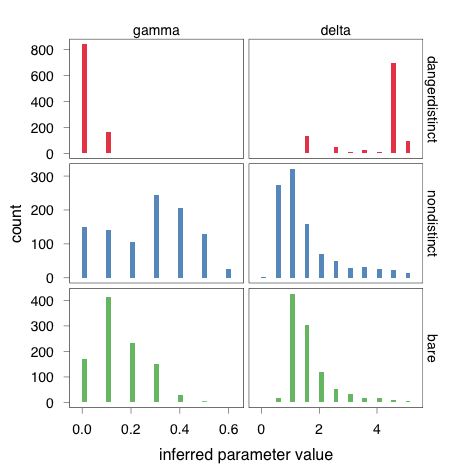
\includegraphics[width=\columnwidth]{fig4_bda2_hyper}
%    \caption{Hyperprior parameters for lifted-variable RSA model}
%  \label{fig:bda2hyperparams}
%\end{figure}

We use this data analysis model to infer the hyperprior parameter values for the Lifted-variable RSA model. Figure \ref{fig:modeldatapriors} (bottom) shows prior distributions from the posterior mean inferred values of the hyperprior parameters. This makes the prediction that, if this were the correct model of human cognition, the prior distribution of the \emph{dangerous \& distinctive} condition would be heavily skewed towards lower prevalence levels. This makes sense insofar as a distinctive feature is one that is relatively rare. Our intuitions are again confirmed in the inferred distribution of the \emph{nondistinctive} context. A nondistinctive feature is one that is very common. The prior distribution of the \emph{bare} context lies somewhere in between these two extremes: neither distinctive nor nondistinctive.

The posterior predictive distributions marginalizes over the hyperprior parameters to produce predictions about what the data should look like given the cognitive model and the inferred data. This is an important step in model validation as it shows what the model actually predicts the data should look like \footnote{As a thought experiment, consider 2 coins assumed to come from a single coin-making machine. You flip each 100 times. The first one returns 100 heads, and the second one returns 100 tails. The posterior mean of the inferred coin weight will be 0.5. Comparing the posterior predictive distribution (based on this inferred coin-weight) to the observed data will highlight the fact that your theory about the ``single coin-making machine'' is seriously flawed.}.The predictions for the lifted variable RSA model are in Figure \ref{fig:bda1posteriorpred} (right). We can see here that model predicts intermediate endorsement rates for the generic at lower prevalence levels. In a sense, the model has some persistent uncertainty about the true value of the threshold, a feature that people share. We reconstruct the curves of Figure \ref{fig:replication} well; the model--data correlation is $r = 0.97$.

It should also be noted that the mean inferred value of  \lstinline{phi} is about 0.2, a seemingly reasonable estimation of ``guessing'' probability for participants on Amazon's Mechanical Turk.

%\begin{figure}
%\centering
%    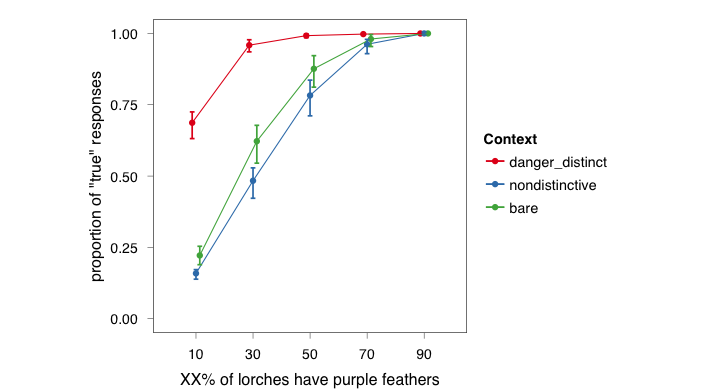
\includegraphics[width=\columnwidth]{fig5_bda2_postpred}
%    \caption{Posterior predictive using lifted-variable RSA}
%  \label{fig:postpred2}
%\end{figure}

In addition to making predictions about the proportion of ``true'' responses to generic statement under different prevalence levels, the combination of the RSA model of language understanding and the bayesian data analysis model gives rise to predictions about the shape of the prior distribution of prevalence levels under different contexts. We take these predictions seriously and test these in a second experiment. 

\section{Experiment 2}

Exp. 2 sought to test the prediction that the prior distribution of prevalence levels would vary by context, as predicted by the $\gamma$ and $\delta$ data analysis parameters from the previous section.

\subsection{Method}

\subsubsection{Participants}

We recruited 30 participants over Amazon's crowd-sourcing platform Mechanical Turk. 

\subsubsection{Procedure and materials}

Our procedure was identical to Experiment 1 in all aspects except the question that was asked of the participant\footnote{The experiment in full can be viewed at \url{http://stanford.edu/~mtessler/experiments/generics/cbg2010-replication/experiment/experiment-8.html}}. 

In addition to the prevalence and contextual information, participants were presented with the following additional piece of information ``The island has 100,000 other animals on it.'' and asked the following question: ``How many other animals do you think have purple feathers?''

\subsubsection{Results}

Experiment 2 recovered the shape of the inferred prior distributions from the lifted variable RSA (Figure \ref{fig:modeldatapriors}).


\begin{figure}
\centering
    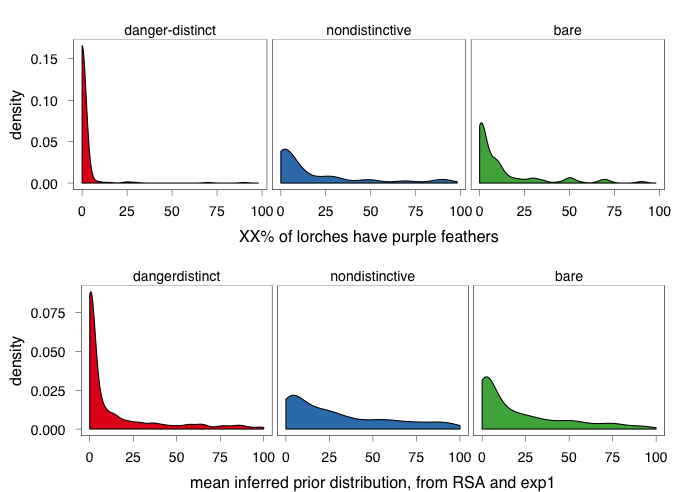
\includegraphics[width=\columnwidth]{exp2densities_inferredMeanPriorExp1}
    \caption{Prior distributions over prevalence. Elicited via Experiment 2 (top). Inferred from Bayesian model (bottom).}
  \label{fig:modeldatapriors}
\end{figure}


\section{Asymmetries in dependent measures}

CBG showed how contexts affects the endorsement for generic statements. An additional concern of their experiments surrounded the relation between two dependent measures for understanding generics. One dependent measure was the ``truth conditions'', or \emph{sentence verification} measure that we've been considering up to this point. The other was an ``implied prevalence'', or \emph{sentence interpretation} dependent measure. The latter was collected by giving participants the generic statement (plus, any additional contextual information), and asking the participant ``What percentage of lorches have purple feathers?''

In their analysis, they found that the quantifier ``most'' expressed a symmetry between the two dependent measures, while the generic had an asymmetry\footnote{This asymmetry has since been replicated in adults and observed in children \cite{Brandone2014}}. In this section, we show how you can recover an asymmetry between these dependent measures by considering communicative roles and Questions Under Discussion (QUDs).

\subsection{Speak and listen}

\citeA{Degen2014} argued that differences between dependent measures in experimental effects of pragmatic inference can be accounted for by formal, probabilistic models of pragmatics. In particular, they suggest the \emph{sentence verification} measure is most closely related to production, and should therefore be modeled as a speaker. Additionally, \emph{sentence interpretation} was shown to be best accounted for by a model of a listener. We apply this same logic to the CBG paradigm to show how the asymmetry can come about from these different dependent measures.

Figure \ref{fig:asymmetry} \red{doesn't show what we want it to show... yet}.



\section{Discussion}

We have shown how a Bayesian model of language understanding, motivated by contextual variation of the effective threshold of the generic statement, can explain the data. We have used technique in Bayesian data analysis to help arbitrate between two cognitive theories. The first was a simple theory that proposed that a generic was akin to some alien quantifier. This quantifier behaves like other quantifiers in that it has a fixed-threshold semantics. The only thing special about the generic is that the threshold is different for different contexts. We believe this is a tacit assumption of many approaches, but that this assumption lay hidden behind NHST of semantic content.

\begin{figure}
\centering
    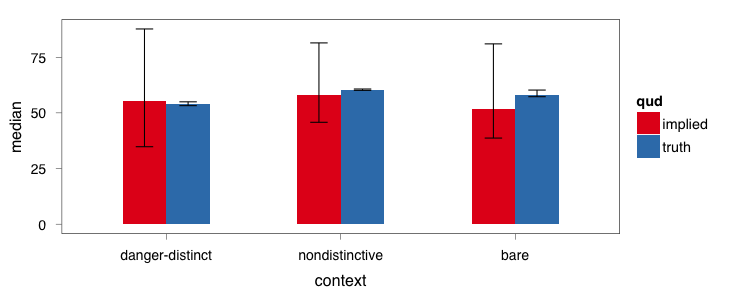
\includegraphics[width=\columnwidth]{exp9_postpred_speakListen_asymmetry}
    \caption{Symmetries and asymmetries among dependent measures and quantifiers.}
  \label{fig:asymmetry}
\end{figure}

The alternative theory was that there is no known generic-threshold, even within a given context. There is only uncertainty, and though that uncertainty may be reduced by further contextual information, it never completely evaporates. Instead, we are only left with a posterior belief distribution over possible thresholds as well as a posterior belief distribution over possible worlds. 

In this paper, we used techniques of both Bayesian Cognitive Science and Bayesian Data Analysis. The former helped us develop a rich, formal theory of language understanding. These sorts of theories have implications for psychology and linguistics. The latter helped us make inferences about our theories. Bayesian Data Analysis is crucial to make assumptions explicit (e.g. about fixed-threshold semantics) and clean up our data (e.g. discounting behavior that can conceivably be attributed to guessing). Together, they embody a manifestation of a more general philosophy of science: making assumptions explicit and beginning our science by announcing our uncertainty.

What we're left is an explanation that not all pieces of language need definite semantic content. Mr. Obama's proclamation and the very fact that he went through the trouble to say it suggests that perhaps many members of Congress are able to talk to each other. From another angle, though, 
we can use our knowledge of the world---and the Union---to determine that ``Members of both parties'' supporting Mr. Obama is probably a pretty rare feature; perhaps it would be distinctive of our time (relative to the past). By this logic, the threshold for validly producing the generic could be quite low.  But maybe we shouldn't spend so much energy inferring the threshold, and instead, listen to hear what his other words may suggest.

%\begin{itemize}
%
%\item Replace figure 4 (hyperprior parameters) with mean distribution?
%
%\item Collapse Figure 3 \& 5 (posterior predictive) into one
%
%\item Exp 2 to confirm $\gamma$ and $\delta$. 
%
%\item Some linking function to condition on Exp 1 \& 2 simultaneously,  to perhaps, infer rationality parameter and get some posterior predictives.
%
%\end{itemize}
%
%The data analysis involved comparing the mean of the prevalence ratings associated with \emph{True} endorsements of the generic with the mean prevalence ratings elicited by the generic in a separate task. In the experimental pragmatics literature, the dependent measure involved in the ``truth conditions'' task is called \emph{sentence verification}; in the ``implied prevalence'' task, it is a \emph{sentence interpretation}. 
%
%These different dependent measures, we argue, imply different Questions Under Discussion (QUD, \cite{Roberts2004}). 



%	\section{Sentence verification is a speaker task}
%	
%	DegenGoodman2014.  Truth conditions task --> QUD = ``generic true?'' Model.
%	
%	But what is the semantics of the generic? \citeA{Cimpian2010}, experiments 1, 3, and 4 found that the truth conditions of the generic are sensitive to the context.  Our goal is to replicate this finding, and use Bayesian data analysis to infer the threshold of the speaker model. This bears some similarity to Michael Franke's approach for cogsci from last year.
%	
%	
%	
%	
%	\section{The full bayesian thing}
%	
%	Computational models of cognition typically have parameters. Many of these parameters are of theoretically interest, because they are posited to reside within the head of the subject.
%	
%	\subsection{Inferring quantifier threshold by context}
%	
%	Here we'll find that the generic threshold changes by context. We might also want to show that ``most'' and ``some'' do not change by context.
%	
%	\subsection{Are generics like adjectives?}
%	
%	To determine if a generic is true or false, we must refer to context. The threshold in the threshold-semantic view of the statement varies by context. This property has been shown to be an important feature in the semantics of gradable adjectives (e.g. \emph{tall}) \cite{Lassiter2014}.  
%	
%	\section{Lifted-variable speech act model}
%	
%	We can start in a single context, with a uniform prior over states. We can look at the posterior over states, for listener1. As well, we can look at the posterior over thetas. This depends of course on the alternatives, for which we may want to consider only the experimental alternatives \emph{some, most, generic} or for which we may want to include \emph{all}.  Either way, here we'll recreate the asymmetry between listener and speaker --- between implied prevalence and truth conditions. 
%	
%	\citeA{Cimpian2010} report a ``paradoxical asymmetry at the core of generic meaning'' which manifests as the generic having ``extremely strong implications but requiring little evidence to be judged true''. Here, we explain this ``paradox'' by the different Questions Under Discussions in the tasks used and by the different roles intrinsic to speech-acts: the role of the speaker and the role of the listener. 
%	
%	\subsection{Questions Under Discussion in two tasks}
%	
%	\citeA{Cimpian2010} used two tasks (with different dependent measures) to get at the comparison between ``acceptance'' and ``implications''. These two tasks --- called ``truth conditions'' and ``implied prevalence'' -- used different questions and different dependent measures to get at the meaning of generics. In the ``truth conditions'' task, subjects are given evidence about the prevalence of a property (e.g. ``50\% of morseths have silver fur'') and are asked to judge the corresponding generic (i.e. ``Morseths have silver fur'') to be either true or false. In the ``implied prevalence'' task, subjects are given a generic statement and asked ``What percentage of morseths do you think have silver fur?''
%	
%	\citeA{Degen2014} argue that the \emph{sentence verification} (``truth conditions'') task should be modeled as a speaker task, and that the \emph{sentence interpretation} (``implied prevalence'') task should be modeled as a listener task. In addition to different communicative roles, there are also different implicit Questions Under Discusision. In the ``truth conditions'' task, the QUD seems to be ``is the generic true or false?'', whereas in the ``implied prevalence'' task, the QUD seems to be ``what percentage of category X have property Y?''.







%
%\section{General Formatting Instructions}
%
%The entire contribution of a proceedings paper (including figures,
%references, and anything else) can be no longer than six pages.
%
%The text of the paper should be formatted in two columns with an
%overall width of 7 inches (17.8 cm) and length of 9.25 inches (23.5
%cm), with 0.25 inches between the columns. Leave two line spaces
%between the last author listed and the text of the paper. The left
%margin should be 0.75 inches and the top margin should be 1 inch.
%\textbf{The right and bottom margins will depend on whether you use
%  U.S. letter or A4 paper, so you must be sure to measure the width of
%  the printed text.} Use 10~point Times Roman with 12~point vertical
%spacing, unless otherwise specified.
%
%The title should be in 14~point, bold, and centered. The title should
%be formatted with initial caps (the first letter of content words
%capitalized and the rest lower case). Each author's name should appear
%on a separate line, 11~point bold, and centered, with the author's
%email address in parentheses. Under each author's name list the
%author's affiliation and postal address in ordinary 10~point type.
%
%Indent the first line of each paragraph by 1/8~inch (except for the
%first paragraph of a new section). Do not add extra vertical space
%between paragraphs.
%
%
%\section{First Level Headings}
%
%First level headings should be in 12~point, initial caps, bold and
%centered. Leave one line space above the heading and 1/4~line space
%below the heading.
%
%
%\subsection{Second Level Headings}
%
%Second level headings should be 11~point, initial caps, bold, and
%flush left. Leave one line space above the heading and 1/4~line
%space below the heading.
%
%
%\subsubsection{Third Level Headings}
%
%Third level headings should be 10~point, initial caps, bold, and flush
%left. Leave one line space above the heading, but no space after the
%heading.
%
%
%\section{Formalities, Footnotes, and Floats}
%
%Use standard APA citation format. Citations within the text should
%include the author's last name and year. If the authors' names are
%included in the sentence, place only the year in parentheses, as in
%\citeA{NewellSimon1972a}, but otherwise place the entire reference in
%parentheses with the authors and year separated by a comma
%\cite{NewellSimon1972a}. List multiple references alphabetically and
%separate them by semicolons
%\cite{ChalnickBillman1988a,NewellSimon1972a}. Use the
%``et~al.'' construction only after listing all the authors to a
%publication in an earlier reference and for citations with four or
%more authors.
%
%
%\subsection{Footnotes}
%
%Indicate footnotes with a number\footnote{Sample of the first
%footnote.} in the text. Place the footnotes in 9~point type at the
%bottom of the column on which they appear. Precede the footnote block
%with a horizontal rule.\footnote{Sample of the second footnote.}
%
%
%\subsection{Tables}
%
%Number tables consecutively. Place the table number and title (in
%10~point) above the table with one line space above the caption and
%one line space below it, as in Table~\ref{sample-table}. You may float
%tables to the top or bottom of a column, or set wide tables across
%both columns.
%
%\begin{table}[!ht]
%\begin{center} 
%\caption{Sample table title.} 
%\label{sample-table} 
%\vskip 0.12in
%\begin{tabular}{ll} 
%\hline
%Error type    &  Example \\
%\hline
%Take smaller        &   63 - 44 = 21 \\
%Always borrow~~~~   &   96 - 42 = 34 \\
%0 - N = N           &   70 - 47 = 37 \\
%0 - N = 0           &   70 - 47 = 30 \\
%\hline
%\end{tabular} 
%\end{center} 
%\end{table}
%
%
%\subsection{Figures}
%
%All artwork must be very dark for purposes of reproduction and should
%not be hand drawn. Number figures sequentially, placing the figure
%number and caption, in 10~point, after the figure with one line space
%above the caption and one line space below it, as in
%Figure~\ref{sample-figure}. If necessary, leave extra white space at
%the bottom of the page to avoid splitting the figure and figure
%caption. You may float figures to the top or bottom of a column, or
%set wide figures across both columns.
%
%\begin{figure}[ht]
%\begin{center}
%\fbox{CoGNiTiVe ScIeNcE}
%\end{center}
%\caption{This is a figure.} 
%\label{sample-figure}
%\end{figure}
%
%
%\section{Acknowledgments}
%
%Place acknowledgments (including funding information) in a section at
%the end of the paper.
%
%
%\section{References Instructions}
%
%Follow the APA Publication Manual for citation format, both within the
%text and in the reference list, with the following exceptions: (a) do
%not cite the page numbers of any book, including chapters in edited
%volumes; (b) use the same format for unpublished references as for
%published ones. Alphabetize references by the surnames of the authors,
%with single author entries preceding multiple author entries. Order
%references by the same authors by the year of publication, with the
%earliest first.
%
%Use a first level section heading, ``{\bf References}'', as shown
%below. Use a hanging indent style, with the first line of the
%reference flush against the left margin and subsequent lines indented
%by 1/8~inch. Below are example references for a conference paper, book
%chapter, journal article, dissertation, book, technical report, and
%edited volume, respectively.
%
%\nocite{ChalnickBillman1988a}
%\nocite{Feigenbaum1963a}
%\nocite{Hill1983a}
%\nocite{OhlssonLangley1985a}
%% \nocite{Lewis1978a}
%\nocite{Matlock2001}
%\nocite{NewellSimon1972a}
%\nocite{ShragerLangley1990a}
%

\bibliographystyle{apacite}

\setlength{\bibleftmargin}{.125in}
\setlength{\bibindent}{-\bibleftmargin}

\bibliography{generics}


\end{document}
